In der algebraischen Topologie ist es oft relativ einfach, die Homotopiegruppen gezielt zu eliminieren. Betrachte hierzu einen CW-Komplex \(X\) und ein \(\eqcl{\gamma}\in\pi_k(X)\). Dann ergibt das Ankleben einer \((k+1)\)-Zelle entlang der Anklebeabbildung \(\gamma\colon\mathbb{S}^k\to X\) einen CW-Komplex, in welchem \(\gamma\) nullhomotop ist. Die niederen Homotopiegruppen bleiben hierbei gleich, die h\"oheren Homotopiegruppen nicht zwingenderma\ss en. Dieser Prozess versagt f\"ur Mannigfaltigkeiten (insbesonders glatte) auf ganzer Linie. Eine pr\"azise Formulierung einer Verklebung f\"ur glatte Mannigfaltigkeiten l\"asst sich als \textit{etwas haarig} beschreiben. Der naive Ansatz die Verklebung zweier glatte Mannigfaltigkeiten \(\mathcal{M}\) und \(\mathcal{N}\) entlang einer eingebetteten Mannigfaltigkeit \(\mathcal{S}\) \"uber das topologisches Pushout-Diagramm
\begin{center}
    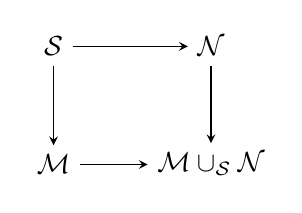
\begin{tikzpicture}
        \draw   (0, 0) node (A) {\(\mathcal{S}\)}
                (0, -1.5) node (B) {\(\mathcal{M}\)}
                (2, 0) node (C) {\(\mathcal{N}\)}
                (2, -1.5) node (D) {\(\mathcal{M}\cup_{\mathcal{S}}\mathcal{N}\)}
                
                (A) edge [-stealth] (B)
                (A) edge [-stealth] (C)
                (B) edge [-stealth] (D)
                (C) edge [-stealth] (D)
                ;
    \end{tikzpicture}
\end{center}
\noindent zu definieren birgt allgemein keinen lokal euklidischen Raum. Selbst wenn sich eine topologische Mannigfaltigkeit ergibt, ist dies keine glatte Mannigfaltigkeit sondern eine \textit{glatte Mannigfaltigkeit mit Ecken}. Diese k\"onnen zwar gegl\"attet werden (siehe Abbildung \ref{fig:smooth_corner}), was jedoch nicht sonderlich elegant ist und eine Reihe von weiteren Problemen einf\"uhrt. F\"ur die korrekte Verklebung m\"ussen unterschiedliche F\"alle unterschieden werden, die Vorgehensweise ist jedoch stets gleich. Seien \(\mathcal{M}\) und \(\mathcal{N}\) Mannigfaltigkeiten mit einer gemeinsamen Untermannigfaltigkeit \(\mathcal{V}\). Dann entstehe die Verklebung von \(\mathcal{M}\) und \(\mathcal{N}\) entlang von \(\mathcal{V}\) durch das Identifizieren von Tubenumgebungen von \(\mathcal{V}\) in \(\mathcal{M}\) und \(\mathcal{N}\) \"uber einen orientierungsumkehrenden Diffeomorphismus. Das Problem besteht darin, dass abgesehen von der Position von \(\mathcal{V}\) in \(\mathcal{M}\) und \(\mathcal{N}\) unterschiedliche Begriffe von Tubenumgebungen betrachtet werden m\"ussen. F\"ur alle n\"otigen Eindeutigkeitsbeweise siehe \cite{kosinski1992differential} Kapitel VI Sektionen 1-5.

\subsection{Tubenumgebungen}
    Sei \(\mathcal{V}^k\hookrightarrow\mathcal{M}^n\) eine Untermannigfaltigkeit. Die folgenden drei Positionen von \(\mathcal{V}\) in \(\mathcal{M}\) sind m\"oglich und am einfachsten zu handhaben.
    \begin{enumerate}
        \item \(\mathcal{V}\subseteq\mathring{\mathcal{M}}\) ist geschlossen,
        \item \(\mathcal{V}\subseteq\partial\mathcal{M}\) ist geschlossen,
        \item \((\mathcal{V},\partial\mathcal{V})\subseteq(\mathcal{M},\partial\mathcal{M})\) ist eine ordentliche Untermannigfaltigkeit.
    \end{enumerate}
    Insbesondere sind auch drei unterschiedliche Begriffe von Tubenumgebungen erforderlich. Siehe Abbildung \ref{fig:tub_neigh}.

    \begin{figure}[t]
        \centering
        \begin{minipage}[t]{.45\textwidth}
            \centering
            \begin{tikzpicture}[scale = 1.3]
                \draw [rounded corners, pattern = north west lines] (0, 0) -- (1, 0) -- (1, 1) -- (0, 1) -- cycle;
                \draw [pattern = north east lines] (1, 0.25) node {\textcolor{red}{\tiny\textbullet}} arc (-90:180:0.75) node {\textcolor{red}{\tiny\textbullet}} -- (0.75, 1) node {\textcolor{red}{\tiny\textbullet}} arc (180:-90:0.25) node {\textcolor{red}{\tiny\textbullet}} -- cycle;
                \begin{scope}[xshift = 2cm]
                    \draw [rounded corners, pattern = north east lines] (0, 0) -- (1, 0) -- (1, 0.25) arc (-90:180:0.75) -- (0, 1) -- cycle;
                    \draw [rounded corners = 0.75, draw = black, fill = white] (1, 1) -- (1, 0.75) arc (-90:180:0.25) -- cycle;
                \end{scope}
            \end{tikzpicture}
            \caption{Abrunden der Ecken durch eine Hom\"oomorphie.}\label{fig:smooth_corner}
        \end{minipage}\hfill
        \begin{minipage}[t]{.52\textwidth}
            \centering
            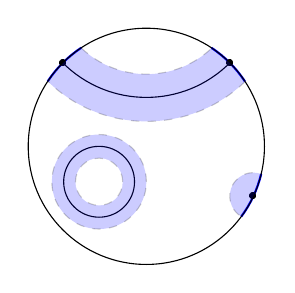
\begin{tikzpicture}[scale = 1.5]
                \draw [blue, thick]
                    (146.5207:1) arc (146.5207:123.448:1)
                    (56.551:1) arc (56.4509:33.27295:1)
                    (-13.522:1) arc (-13.522:-36.478:1)
                ;
                \draw 
                    (0:1) arc (0:360:1)
                    (45:1) node {\tiny\textbullet} arc (-45:-135:1) node {\tiny\textbullet}

                    (-0.1, -0.3) arc (0:360:0.3)
                    (-25:1) node {\tiny\textbullet}
                ;
                \draw [fill = blue, opacity = 0.2, dashed]
                    (33.27295:1) arc (-45.963:-134.037:1.2)
                    arc (146.5207:123.448:1)
                    arc (-133.5491:-46.4509:0.8)
                    arc (56.4509:33.27295:1) -- cycle
                ;
                \draw [fill = blue, opacity = 0.2, dashed]
                    (-13.522:1) arc (-13.522:-36.478:1)
                    arc (239.2608:70.739:0.2) --cycle
                ;
                \draw [fill = blue, opacity = 0.2, dashed] (0, -0.3) arc (0:360:0.4);
                \fill [white, dashed] (-0.2, -0.3) arc (0:360:0.2);
                \draw [opacity = 0.2, dashed] (-0.2, -0.3) arc (0:360:0.2);
            \end{tikzpicture}
            \caption{Die drei unterschiedlichen Arten von Tubenumgebungen in \(\mathbb{D}^2\).}\label{fig:tub_neigh}
        \end{minipage}
    \end{figure}


    \subsubsection{Untermannigfaltigkeiten des Inneren}
        Sei \(\iota\colon\mathcal{V}^k\hookrightarrow\mathring{\mathcal{M}}\) eine geschlossene Untermannigfaltigkeit und \(0\colon\mathcal{V}\to N\mathcal{V}\) der Nullschnitt. 
        \begin{definition}[Tubenumgebung f\"ur \(\mathcal{V}\subseteq\mathring{\mathcal{M}}\)]
            Ein riemannsches Vektor\-b\"un\-del \(\xi\colon E\to\mathcal{V}\) vom Rang \(n-k\) und eine Einbettung \(\Psi\colon E\hookrightarrow\mathring{\mathcal{M}}\) sodass \(\Psi\circ0=\iota\) ist.
        \end{definition}
        \noindent Es ist ein Standardresultat, dass derartige Tubenumgebungen existieren, bis auf Isotopie eindeutig bestimmt sind und \(\xi\) zu dem Normalenb\"undel isomorph ist.

    \subsubsection{Untermannigfaltigkeiten des Randes}
        Sei \(\iota\colon\mathcal{V}^k\hookrightarrow\partial\mathcal{M}^{n+1}\) eine geschlossene Untermannigfaltigkeit.
        \begin{definition}[Tubenumgebung f\"ur \(\mathcal{V}\subseteq\partial\mathcal{M}\)]
            Eine Tubenumgebung \({\Psi\colon E\hookrightarrow\partial\mathcal{M}}\) mit einer Fortsetzung zu einer Einbettung \({\Tilde{\Psi}\colon E\times\mathbb{R}_+\hookrightarrow\mathcal{M}}\).
        \end{definition}
        \noindent Eine derartige Tubenumgebung l\"asst sich mithilfe von einer Tubenumgebung in \(\partial\mathcal{M}\) und  einer Kragenumgebung \(\partial\mathcal{M}\times\mathbb{R}_+\hookrightarrow\mathcal{M}\) konstruieren und ist somit erneut bis auf Isotopie eindeutig bestimmt. Beachte hierbei, dass das Normalenb\"undel von \(\mathcal{V}\) in \(\mathcal{M}\) kein \textit{Halbraumb\"undel}, sondern ein normales \((n-k)\)-dimensionales Vektorb\"undel ist, weshalb nicht einfach eine Einbettung des Normalenb\"undels von \(\mathcal{V}\) in \(\mathcal{M}\) gew\"ahlt werden kann.

    \subsubsection{Ordentliche Untermannigfaltigkeiten}
        Eine Untermannigfaltigkeit \(\mathcal{V}\subseteq\mathcal{M}\) hei\ss e ordentliche Untermannigfaltigkeit (neat submanifold), wenn:
        \begin{itemize}
            \item[i] Es gelte \(\partial\mathcal{V}=\mathcal{V}\cap\partial\mathcal{M}\)
            \item[ii] F\"ur alle \(p\in\partial\mathcal{M}\) existiert eine Karte \(\alpha\colon\mathbb{R}_+^n\to U\) mit \(\alpha\mathbb{R}_+^k=U\cap\mathcal{V}\).
        \end{itemize}
        \begin{definition}[Ordentliche Tubenumgebung]
            Ein riemannsches Vektor\-b\"un\-del \(\xi\colon E\to\mathcal{V}\) mit einer Einbettung \(\tilde{\Psi}\colon E\hookrightarrow\mathcal{M}\) die mit \(\iota\) kommutiert, sodass die Einschr\"ankung \(\Psi\colon E|_{\partial\mathcal{V}}\hookrightarrow\partial\mathcal{M}\) eine Tubenumgebung von \(\partial\mathcal{V}\) in \(\partial\mathcal{M}\) ist.
        \end{definition}

\subsection{Die Randsumme}
    Die Summe zweier Mannigfaltigkeiten ist stets die gleiche, auch wenn die Tubenumgebungen etwas unterschiedliche Formen besitzen. Die Konstruktion sei hier nur an der Randsumme erl\"autert, die anderen beiden F\"alle verlaufen analog. Sei \({\xi\colon E\to\mathcal{V}}\) ein riemannsches Vektorb\"undel und f\"ur \({i\in\{1,2\}}\) jeweils \({\mathcal{M}_i}\) Mannigfaltigkeiten, \({\iota_i\colon\mathcal{V}\hookrightarrow\partial\mathcal{M}_i}\) Untermannigfaltigkeiten mit Tubenumgebungen \({\psi_i\colon E\hookrightarrow\partial\mathcal{M}_i}\) in \({\partial\mathcal{M}_i}\). Seien \({\Psi_i\colon E\times\mathbb{R}_+\hookrightarrow\mathcal{M}_i}\) Fortsetzungen der \({\psi_i}\) zu Tubenumgebungen in \({\mathcal{M}_i}\). Sei zuletzt die diffeomorphe Involution
    \[\alpha\colon(E\times\mathbb{R}_+)\setminus\mathbf{0}\to(E\times\mathbb{R}_+)\setminus\mathbf{0},\,v\mapsto\frac{v}{\norm{v}^2}\]
    gegeben, so identifiziere
    \[\Psi_1(x)\sim\Psi_2\alpha(x)\quad\forall x\in(E\times\mathbb{R}_+)\setminus\mathbf{0}\,,\]
    und setze
    \[\mathcal{M}_1\mathop{+}_{\Psi_1}^{\Psi_2}\mathcal{M}_2=\left(\mathcal{M}_1\setminus\iota_1(\mathcal{V})\sqcup-\mathcal{M}_2\setminus\iota_2(\mathcal{V})\right)/\sim\,.\]
    Diese Konstruktion ist bis auf Diffeomorphie unabh\"angig von der Wahl der Fortsetzung der \({h_i}\). Weiter ergeben isotope Einbettungen diffeomorphe Mannigfaltigkeiten. Beachte, dass unterschiedliche \(\Psi\) allgemein jedoch sehr wohl den Diffeomorphietyp der Summe ver\"andern kann.

    \subsubsection{Die verbundene Summe}
        Ein Spezialfall tritt auf, wenn \(\mathcal{V}\) ein Punkt ist. In diesem Fall wird die Summe zweier Mannigfaltigkeiten auch verbundene Summe genannt. Siehe Abbildung \ref{fig:conn_sum}.
        \begin{figure}
            \centering
            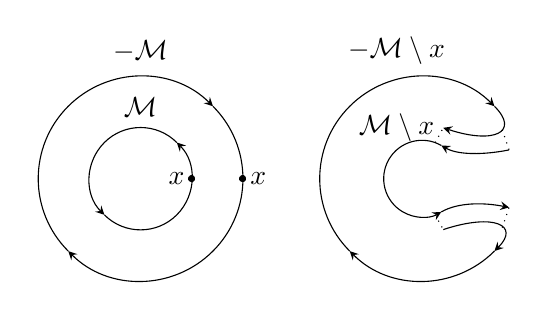
\begin{tikzpicture}[scale = 0.65]
                \begin{scope}[xshift = -2cm]
                    \draw [-stealth] (45:1) arc (45:225:1);
                    \draw [-stealth] (-135:1) arc (-135:45:1);
                    \draw (1, 0) node {\tiny\textbullet} ++(-0.3, 0) node {\(x\)};
                    
                    \draw [-stealth] (225:2) arc (225:45:2);
                    \draw [-stealth] (45:2) arc (45:-135:2);
                    \draw (2, 0) node {\tiny\textbullet} ++(0.3, 0) node {\(x\)};

                    \draw (0, 1.4) node {\(\mathcal{M}\)};
                    \draw (0, 2.5) node {\(-\mathcal{M}\)};
                \end{scope}
                
                \begin{scope}[xshift = 3.5cm]
                    \draw [-stealth] 
                        (60:0.75) arc (60:300:0.75);
                    \draw [-stealth] 
                        (225:2) arc (225:45:2);
                    \draw [-stealth]
                        (45:2) node (A) {}
                        ++(0.5, -0.5) node (B) {}
                        ++(-0.5, -0.25) node (C) {}
                        ++(-1, 0.33) node (D) {}
                        (A.center) .. controls (B.center) and (C.center) .. (D.center) node [pos = 0.4] (BB) {}
                        ;
                    \path
                        (-45:2) node (H) {}
                        ++(0.5, 0.5) node (G) {}
                        ++(-0.5, 0.25) node (F) {}
                        ++(-1, -0.33) node (E) {};
                    \draw [-stealth]
                        (E.center) .. controls (F.center) and (G.center) .. (H.center) node [pos = 0.6] (AA) {};
                    \draw [-stealth] (H) arc (-45:-135:2);
                    \draw [-stealth] (60:0.75) node (I) {}
                        ++(0.3248, -0.1875) node (J) {}
                        ++(0.5, 0) node (K) {}
                        ++(0.5, 0.1) node (L) {}
                        (L.center) .. controls (K.center) and (J.center) .. (I.center)
                    ;
                    \draw [-stealth] (-60:0.75) node (M) {}
                        ++(0.3248, 0.1875) node (N) {}
                        ++(0.5, 0) node (O) {}
                        ++(0.5, -0.1) node (P) {}
                        (M.center) .. controls (N.center) and (O.center) .. (P.center)
                    ;
                    
                    \draw [dotted] 
                        (290:0.75) -- (E.center)
                        (70:0.75) -- (D.center)
                        (AA.center) -- (P.center)
                        (BB.center) -- (L.center)
                        (-0.5, 1) node {\(\mathcal{M}\setminus x\)} 
                        (-0.5, 2.5) node {\(-\mathcal{M}\setminus x\)};
                \end{scope}
            \end{tikzpicture}\hfill
            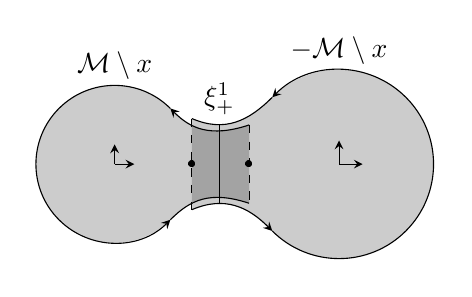
\begin{tikzpicture}[scale = 0.5]
                    \draw 
                        (45:2) node (A) {}
                        ++(0.5, -0.5) node (B) {}
                        ++(0.5, -0.25) node (C) {}
                        ++(1, 0.33) node (D) {}
                        
                        (-45:2) node (H) {} 
                        ++(0.5, 0.5) node (G) {}
                        ++(0.5, 0.25) node (F) {}
                        ++(1, -0.33) node (E) {}

                        (0, 2.5) node {\(\mathcal{M}\setminus x\)}
                        ;
                    \draw [-stealth] (D.center) .. controls (C.center) and (B.center) .. (A.center);
                    \draw [-stealth] (A.center) arc (45:315:2);
                    \draw (315:2) .. controls (G.center) and (F.center) .. (E.center); % Large lower
                    \draw [-stealth] (0, 0) -- (0, 0.5); 
                    \draw [-stealth] (0, 0) -- (0.5, 0);
                    \fill [opacity = 0.2] (D.center) .. controls (C.center) and (B.center) .. (A.center) arc (45:315:2) .. controls (G.center) and (F.center) .. (E.center) -- cycle;
                    \begin{scope}[xshift = 5.7cm, scale = 1.2]
                        \draw [-stealth] (-135:2) arc (-135:135:2);
                        \draw (135:2) node (A1) {}
                            ++(-0.5, -0.5) node (B1) {}
                            ++(-0.5, -0.25) node (C1) {}
                            ++(-0.7, 0.3) node (D1) {}
                            
                            (-135:2) node (E1) {}
                            ++(-0.5, 0.5) node (F1) {}
                            ++(-0.5, 0.25) node (G1) {}
                            ++(-0.7, -0.3) node (H1) {}
                            
                            (0, 2.4) node {\(-\mathcal{M}\setminus x\)}
                            ;
                        \draw (A1.center) .. controls (B1.center) and (C1.center) .. (D1.center);
                        \draw [-stealth] (H1.center) .. controls (G1.center) and (F1.center) .. (E1.center);
                        
                        \draw [dashed] 
                            (D1.center) -- (H1.center) node [pos = 0.5] {\tiny\textbullet} 
                            (D.center) -- (E.center) node [pos = 0.5] {\tiny\textbullet};
                        \draw [-stealth] (0, 0) -- (0, 0.5); 
                        \draw [-stealth] (0, 0) -- (0.5, 0);
                        \fill [opacity = 0.2] (H1.center) .. controls (G1.center) and (F1.center) .. (E1.center) node (X) [pos = 0.3] {} arc (-135:135:2) .. controls (B1.center) and (C1.center) .. (D1.center) node (XX) [pos = 0.7] {} -- cycle;
                    \end{scope}
                    \draw (X.center) -- (XX.center) node [above] {\(\xi_+^1\)}; 
            \end{tikzpicture}
            \caption{Die verbundenen Summe zweier Kreise und die verbundene Rand\-sum\-me zweier Scheiben.}\label{fig:conn_sum}
        \end{figure}

    \subsection{Homologie von Verklebungen am Rand}
        Sei \(\mathcal{V}^i\) eine gemeinsame Untermannigfaltigkeit der R\"ander von \(\mathcal{M}^n\) und \(\mathcal{N}^n\) mit trivialen Normalenb\"undeln. Seien \(A_1\) und \(A_2\) die Bilder von \(\mathcal{M}\setminus\mathcal{V}\) und \(\mathcal{N}\setminus\mathcal{V}\) in \(\mathcal{M}\mathop{+}^{\mathcal{V}}\mathcal{N}\). Dann ist die zugeh\"orige Mayer-Vietoris Folge von der Form
        \[H_*(A_1\cap A_2)\to H_*(A_1)\oplus H_*(A_2)\to H_*(\mathcal{M}\mathop{+}^{\mathcal{V}}\mathcal{N})\to H_{*-1}(A_1\cap A_2)\,.\]
        Hierbei ist \(A_1\cap A_2\) zu einer Tubenumgebung von \(\mathcal{V}\) isomorph, aus welcher \(\mathcal{V}\) entfernt wurde. Da eine triviale Tubenumgebung in diesem Fall von der Form \(\mathcal{V}\times\mathbb{R}^{n-i-1}\times\mathbb{R}_+\) ist, enth\"alt \({\mathcal{V}\times\mathbb{R}^{n-i-1}\times\mathbb{R}_+\setminus\mathbf{0}}\) den Raum \({\mathcal{V}\times\mathbb{S}_+^{n-i-1}}\) als Deformationsretrakt, also folgt
        \[H_*(A_1\cap A_2)\cong H_*\left(\mathcal{V}\right)\quad\text{und per Ausschneidung}\quad H_*(\mathcal{M},\mathcal{M}\setminus\mathcal{V})=0\,.\]
        Aus \(H_*(\mathcal{M},\mathcal{M}\setminus\mathcal{V})=0\) ergibt sich \(H_*(A_1)\cong H_*(\mathcal{M})\). Die Mayer-Vietoris-Folge ist also
        \[H_*\left(\mathcal{V}\right)\to H_*(\mathcal{M})\oplus H_*(\mathcal{N})\to H_*(\mathcal{M}\mathop{+}^{\mathcal{V}}\mathcal{N})\to H_{*-1}\left(\mathcal{V}\right)\,.\]
        Beispielsweise folgt daraus f\"ur die verbundene Randsumme f\"ur \(j>0\)
        \[H_j(\mathcal{M}+\mathcal{N})\cong H_j(\mathcal{M})\oplus H_j(\mathcal{N})\,.\]
        Beachte, dass dies \textbf{nicht} f\"ur die normale Randsumme entlang des Inneren gilt. In diesem Fall gilt \(H_*(A_1\cap A_2)\cong H_*(\mathbb{S}^{n-1})\), also ist 
        \[H_j(\mathcal{M}+\mathcal{N})\cong H_j(\mathcal{M})\oplus H_j(\mathcal{N})\]
        lediglich f\"ur \(n-1>j>0\). F\"ur orientierte Mannigfaltigkeiten \(\mathcal{M}\) und \(\mathcal{N}\) gilt dies auch f\"ur \(j=n-1\), da der Homomorphismus \(H_n(\mathcal{M}+\mathcal{N})\to H_{n-1}(\mathbb{S}^{n-1})\) dann ein Isomorphismus ist.
        \begin{example}
            Seien \(\mathcal{M}^{2k}\) und \(\mathcal{N}^{2k}\) Mannigfaltigkeiten, die die gleiche Homotopiesph\"are \(\Sigma\) beranden. Dann ist die Verklebung von \(\mathcal{M}\) und \(\mathcal{N}\) entlang \(\Sigma\) eine geschlossene Mannigfaltigkeit, und aus \(H_k(\Sigma)=H_{k-1}(\Sigma)=0\) folgt
            \[H_k(\mathcal{M}\mathop{+}^{\Sigma}\mathcal{N})\cong H_k(\mathcal{M})\oplus H_k(\mathcal{N})\,.\]
        \end{example}
        